

\begin{definition}
A congruence of lines in the plane is a 1d parameter of straight lines.
\end{definition}

 
  % \index[std]{congruence of line}
   In the cartesian form, a congruence is given by:
 

\begin{align}  R(x,y,u)=a(u)x+b(u)y+c(u)=0,\;\; a(u)^2+b(u)^2\ne  0
\label{eq:appB-cr}
\end{align}
It will be assumed that the congruence is of class  $C^k,\, k\geq 3$. 

In general, the equation   $R(x,y,u)=0$ defines a regular surface in   $\mathbb{R}^3$  and its projection   $\pi(x,y,u)=(x,y)$ in the plane is singular in the set  

  \[\mathcal{C}= \{(x,y,u): \; R(x,y,u)=  R_u(x,y,u) =0 \} \]
  which is called the   \textit{criminant set}.
  The projection $\pi(\mathcal{C})$ is called the \textit{envelope} of the congruence. It is also called the     \textit{  discriminant.}
%\index[std]{criminant}
%\index[std]{discriminant}
%\index[std]{envelope}

Te envelope is given by:

\begin{equation}\label{eq:env}
x(u)=\frac{b c^\prime-c b^\prime}{a b^\prime-b a^\prime},\;\;\; y(u)=\frac{c a^\prime-a c^\prime}{a b^\prime-b a^\prime}.
\end{equation}

 

\begin{example}  The envelope of the family of lines defined by   $x \cos u\;  +y\sin u \;  =h(u)$ is the curve
	$E(u)=h(u)(\cos u,\sin u)	+h^\prime(u)(-\sin u, \cos u). $
\end{example}

 
 A congruence of lines, in the parametric form, is given by
 
 \[ x=x_0(t)+v a(t), y=y_0(t)+v b(t)\]

 Therefore, the envelope is given by:
 
	
 	\begin{align*}
   x(t)=&x_0(t)+\frac{   a( b x'_0-a y'_0)}{a b^\prime-b a^\prime} \\
 	y(t)=&y_0(t)+ \frac{   b( b x'_0-a y'_0)}{a b^\prime-b a^\prime} 	\end{align*}
 
 
 
 
 
 Consider a  3-periodic  billiard orbit with vertices $P_i=[x_i(t),y_i(t)]$ (i=1,2,3)
Let $C_i(t)=[1/x_i(t),1/y_i(t)]$. We have that $\{C_1(t),C_2(t),C_3(t)\}$ is a segment. See \cref{exe:chap02-inverse-envelope}.
\begin{proposition}
    The envelope of the family of lines defined by the degenerated polygon $C_i(t)$ (i=1,2,3) is the ellipse $\mathcal{B}$ given by
    \[ {\frac {{a}^{6}{x}^{2}}{ \left( {b}^{2}+\sqrt {{a}^{4}-{a}^{2}{b}^{2}+
{b}^{4}} \right) ^{2}}}+{\frac {{b}^{6}{y}^{2}}{ \left( {a}^{2}+\sqrt 
{{a}^{4}-{a}^{2}{b}^{2}+{b}^{4}} \right) ^{2}}}-1
=0.
    \]
    Moreover, $\mathcal{B}$ is similar to the caustic rotated by $\frac{\pi}{2}.$ See   \cref{fig:appB-inverso-envelope}.
\end{proposition}
 
\begin{proof}
This can be done from the definition of envelope of the family of lines containing the vertices $C_i(t)$.
The calculations are long, but straightforward.
It is helpful to use symbolic computations here. 
\end{proof}

 \begin{figure}
     \centering
     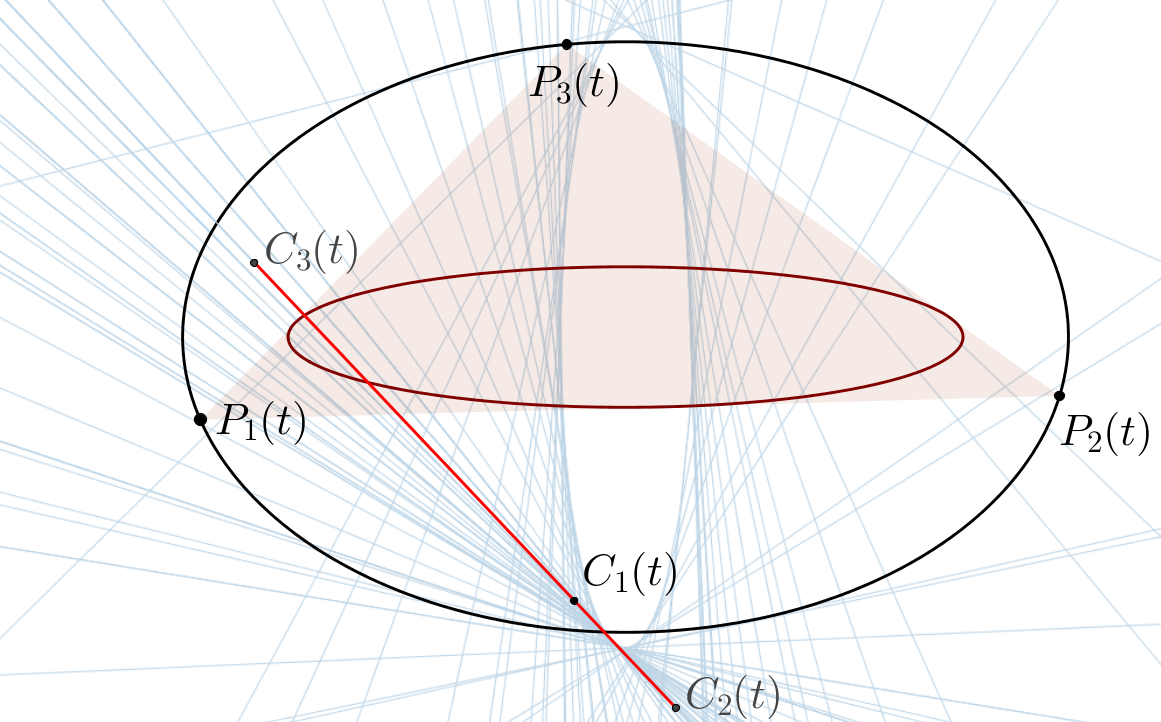
\includegraphics[scale=0.5]{zappB/pics/pics-appB-040inverso_locus_envelope.png}
     \caption{Envelope of the family of lines defined by the degenerated polygons $C_i(t)$}
     \label{fig:appB-inverso-envelope}
 \end{figure}
 
  For more on theory of envelopes see  \cite[Chapter  3]{arnold-1994},  \cite[pp. 305]{berger-1992}, \cite[Chapter   5]{bruce-1992}.  See also \cite[Cap. 1]{carneiro2019-impa}.
  %\cite[Chap{ghys-2017}.  % \cite{kling}. 
 

 

